\documentclass[conference]{IEEEtran}
\IEEEoverridecommandlockouts
% The preceding line is only needed to identify funding in the first footnote. If that is unneeded, please comment it out.
\usepackage{cite}
\usepackage{amsmath,amssymb,amsfonts}
\usepackage{algorithmic}
\usepackage{graphicx}
\usepackage{textcomp}
\usepackage{xcolor}
\usepackage{enumitem}
\usepackage{booktabs}
\usepackage{hyperref}

\def\BibTeX{{\rm B\kern-.05em{\sc i\kern-.025em b}\kern-.08em
    T\kern-.1667em\lower.7ex\hbox{E}\kern-.125emX}}
\begin{document}

% \title{Conference Paper Title*\\
% {\footnotesize \textsuperscript{*}Note: Sub-titles are not captured in Xplore and
% should not be used}
% \thanks{Identify applicable funding agency here. If none, delete this.}
% }

% \author{\IEEEauthorblockN{1\textsuperscript{st} Given Name Surname}
% \IEEEauthorblockA{\textit{dept. name of organization (of Aff.)} \\
% \textit{name of organization (of Aff.)}\\
% City, Country \\
% email address or ORCID}
% \and
% \IEEEauthorblockN{2\textsuperscript{nd} Given Name Surname}
% \IEEEauthorblockA{\textit{dept. name of organization (of Aff.)} \\
% \textit{name of organization (of Aff.)}\\
% City, Country \\
% email address or ORCID}
% \and
% \IEEEauthorblockN{3\textsuperscript{rd} Given Name Surname}
% \IEEEauthorblockA{\textit{dept. name of organization (of Aff.)} \\
% \textit{name of organization (of Aff.)}\\
% City, Country \\
% email address or ORCID}
% \and
% \IEEEauthorblockN{4\textsuperscript{th} Given Name Surname}
% \IEEEauthorblockA{\textit{dept. name of organization (of Aff.)} \\
% \textit{name of organization (of Aff.)}\\
% City, Country \\
% email address or ORCID}
% \and
% \IEEEauthorblockN{5\textsuperscript{th} Given Name Surname}
% \IEEEauthorblockA{\textit{dept. name of organization (of Aff.)} \\
% \textit{name of organization (of Aff.)}\\
% City, Country \\
% email address or ORCID}
% \and
% \IEEEauthorblockN{6\textsuperscript{th} Given Name Surname}
% \IEEEauthorblockA{\textit{dept. name of organization (of Aff.)} \\
% \textit{name of organization (of Aff.)}\\
% City, Country \\
% email address or ORCID}
% }

\title{Towards Transparent Checkpointing with AI-driven Code Generation}

\maketitle

\begin{abstract}
Adding reliable checkpoint/restart support to an MPI scientific application is a time-consuming expert effort that requires deep knowledge of both the application and resilience. We ask whether a frontier large language model can perform this work end-to-end without human intervention. We assemble a benchmark suite of MPI applications spanning diverse domains and computation patterns, and drive an iterative code-generation loop for each application using Anthropic's Claude Opus 4.7 invoked through the OpenCode CLI. Across seventeen scientific applications, the LLM generates working checkpoint/restart code in roughly 45~minutes on average while consuming 5.1~M tokens per application. The generated code adds statistically zero overhead during normal failure-free execution on fourteen of seventeen applications ($\pm 2\%$ of original execution time), and recovers from injected process failures with efficiency comparable to human-engineered checkpoint/restart implementations. These results suggest that automated end-to-end LLM-driven resilience engineering is technically viable today for a meaningful fraction of HPC applications.
\end{abstract}

\begin{IEEEkeywords}
checkpoint/restart, large language models, resilience, HPC, fault tolerance
\end{IEEEkeywords}

\section{Introduction}
\label{sec:intro}

Modern scientific computing combines high performance computing (HPC) and
artificial intelligence (AI) in complex workflows that span heterogeneous infrastructure, from supercomputing centers to scientific instruments. This shift unlocks heterogeneous accelerators and elastic capacity, but also fundamentally reshapes the failure landscape: long-running MPI simulations that once executed on a single homogeneous batch allocation now span resources whose mean-time-between-failure (MTBF) varies significantly; fluctuates dynamically as nodes are preempted, evicted, or reassigned under multi-tenant pressure; and is largely unpredictable at job-submission time~\cite{cappello2014toward,Diaspora-Overview-eScience24}. Under such circumstances, checkpoint/restart, the dominant resilience mechanism in HPC, faces several important challenges:
it is increasingly difficult to identify: (1) which components of the workflow are tightly coupled in ways that let failures propagate rapidly among distributed processes; (2) which data structures within those components are critical and must be protected, and (3) at what point in the code it is safe to checkpoint those data structures. These challenges directly impact the correctness, performance and scalability of checkpoint/restart solutions used to enable resilient execution.

Manual coding of checkpoint/restart solutions to address these challenges can be tedious due to the need to combine performance modeling;
deep understanding of interactions under parallelism to maintain a consistent
global state at scale; fine-tuning; and debugging. Recent advances in large language models (LLMs) and tool-using coding agents~\cite{opencode}, whose performance on bounded software-engineering benchmarks now approaches that of professional developers~\cite{jimenez2024swebench} and whose agentic workflows can autonomously read source trees, plan multi-step transformations, and react to validator feedback, can offer an alternative that is both cheaper to implement and potentially more efficient. The central question of this paper is: \emph{can a frontier LLM coding agent be driven, end-to-end and with no human in the loop, to add production-grade checkpoint/restart resilience to an unmodified MPI scientific application, and at what cost relative to the resulting correctness, performance and scalability?}

\textbf{Key Insights and Contributions.}
This paper investigates the operational viability of \emph{LLM-driven resilience engineering} as a building block for flexible scientific infrastructures. The observation we exploit is that the cognitive work of adding checkpoint/restart (identifying the data structures that make up the critical state, the correct place in the code where to checkpoint it, guarantee global consistency at scale, rebuild other data structures on restart based on the critical state) involves structured reasoning that modern coding agents are well suited for. The trade-off space, however, is far from understood: every iteration of the agent costs millions of tokens and tens of minutes of wall time; conservative state-coverage decisions inflate checkpoint footprint and erode scalability; a misidentified place in the code where it is safe to checkpoint silently corrupts a restart. Our goal is two-fold: (1)~establish empirically that frontier LLM coding agents can produce correct, performant resilience code with no human intervention; and (2)~characterize the cost, correctness and performance trade-offs that determine when this approach is practical for per-deployment resilience synthesis on dynamically provisioned, heterogeneous infrastructures. We summarize our contributions as follows:

\begin{enumerate}[topsep=0pt,itemsep=0pt,leftmargin=12pt]
\item \textbf{End-to-end LLM-driven resilience pipeline:}
We design a closed-loop generate--validate--repair pipeline that drives a frontier coding agent to add VeloC-based checkpoint/restart to an unmodified MPI source tree with no human in the loop. The validator builds the generated code, runs it failure-free, injects a single-rank fault, and structurally checks that the application restarts correctly and reproduces the vanilla output (\S~\ref{sec:setup}).

\item \textbf{Reusable resilience benchmark suite:} We assemble seventeen MPI applications covering diverse domains, code sizes (1K to 627K LOC), state structures, and checkpoint back-ends. Each is shipped with a resilience-stripped \emph{vanilla} source (given to the agent) and an upstream-checkpointed \emph{reference} (human-engineered baseline) (\S~\ref{sec:suite}).

\item \textbf{Empirical characterization of the cost, correctness and performance/scalability trade-off:} We quantify all three axes across the suite. On \emph{cost}, the agent converges in a median of three iterations, averaging 5.1~M tokens and 45~minutes of loop wall time per application. On \emph{correctness}, it consistently identifies a small, sufficient critical-state set and globally safe checkpoint points on every application. On \emph{performance}, the generated code imposes statistically zero failure-free overhead on fourteen of seventeen apps and recovers from injected faults with efficiency comparable to the upstream human-engineered reference (\S~\ref{sec:findings}).
\end{enumerate}


\section{Related Work}

% Established checkpoint/restart approaches such as VeloC~\cite{veloc}, FTI~\cite{fti}, and SCR~\cite{scr} require the developer to manually declare critical state, position checkpoint calls at safe points, and wire restart logic into every initialization path. This is called application-level checkpointing and
% its main advantage is the small size of the checkpoints (only the critical  state), which reduces checkpointing overheads both in terms of performance and storage utilization. These approaches typically rely on \emph{multi-level resilience strategies}~\cite{scr,VELOC-MASCOTS21}: each checkpoint is first staged to a fast node-local tier (RAM or NVMe) for cheap recovery from frequent soft failures, then asynchronously flushed to a slower shared tier (burst buffer, parallel file system), which survives critical failures. A rich body of work optimizes this pipeline: asynchronous flush engines overlap checkpoint I/O with application compute through dedicated background threads or helper agents~\cite{DataStatesLLM-HPDC24,GPUPrefetch-HPDC23}; write aggregation coalesces small per-rank writes into stripe-aligned bulk transfers to relieve parallel-filesystem metadata pressure~\cite{VELOC-FGCS24}; differential and incremental checkpointing persist only the bytes that changed since the previous snapshot~\cite{AICkptHPDC13,GPUDedup-ICPP23}; and on-the-fly compression and lossy encoding further shrink footprint at the cost of a small reconstruction overhead~\cite{SZ-CLUSTER19,LineageComp-HIPC23}. The cadence at which checkpoints are taken is itself an optimization problem: the classical Young~\cite{young1974first}--Daly~\cite{daly2006higher} formulas pick an interval that minimizes expected wasted work as a function of MTBF and checkpoint cost, and adaptive variants extend this model to track fluctuating MTBF on dynamically provisioned, multi-tenant resources~\cite{MLCkpt20}. These mechanisms reduce the cost of resilience at scale, but every one of them presupposes the manual instrumentation step we automate: someone still has to declare what to checkpoint and at which loop point.


% By contrast, transparent checkpointing tools such as BLCR~\cite{blcr}, DMTCP~\cite{dmtcp} and CRIU~\cite{criu}), sidestep developer effort but capture the entire process image, including caches, transient buffers, and rebuildable state. This produces checkpoints orders of magnitude larger than necessary, scales poorly under elasticity, and rarely ports cleanly across heterogeneous nodes. Compiler-assisted approaches~\cite{bronevetsky2003} narrow the snapshot through static analysis but require per-language passes and degrade on the templated, dynamically allocated, irregularly accessed data structures that dominate modern HPC and AI codes. Despite the much larger checkpoint size, such approaches can be complemented with the multi-level resilience strategies mentioned above to partially mitigate the larger checkpointing overheads.

Application-level checkpointing approaches such as VeloC~\cite{veloc}, FTI~\cite{fti}, and SCR~\cite{scr} require developers to manually declare critical state, place checkpoint calls at safe points, and wire restart logic into initialization paths. By saving only the state needed for recovery, they keep checkpoints small and reduce both runtime and storage overhead. These systems typically rely on \emph{multi-level resilience strategies}~\cite{scr,VELOC-MASCOTS21}, where checkpoints are staged to a fast node-local tier, such as RAM, for recovery from frequent soft failures, then asynchronously flushed to a slower shared tier, such as a parallel file system, to survive critical failures.
A rich body of work further optimizes this pipeline: asynchronous flush engines overlap checkpoint I/O with application compute~\cite{DataStatesLLM-HPDC24,GPUPrefetch-HPDC23}; write aggregation coalesces per-rank writes into stripe-aligned bulk transfers~\cite{VELOC-FGCS24}; differential and incremental checkpointing persist only changed bytes~\cite{AICkptHPDC13,GPUDedup-ICPP23}; and compression or lossy encoding reduces footprint at modest reconstruction cost~\cite{SZ-CLUSTER19,LineageComp-HIPC23}. Checkpoint cadence is also optimized: the classical Young~\cite{young1974first}--Daly~\cite{daly2006higher} formulas minimize expected wasted work from MTBF and checkpoint cost, while adaptive variants track fluctuating MTBF on dynamically provisioned, multi-tenant resources~\cite{MLCkpt20}. These mechanisms reduce resilience cost at scale, but still presuppose the manual instrumentation step we automate: someone must decide what to checkpoint and where.

By contrast, transparent checkpointing tools such as BLCR~\cite{blcr}, DMTCP~\cite{dmtcp}, and CRIU~\cite{criu} reduce developer effort by capturing process state automatically, but often include caches, transient buffers, and rebuildable state. This can produce oversized checkpoints, limit scalability under elasticity, and complicate portability across heterogeneous nodes. Compiler-assisted approaches~\cite{bronevetsky2003} narrow the snapshot through static analysis, but require per-language passes and can struggle with the templated, dynamically allocated, irregularly accessed data structures common in modern HPC and AI codes. Although transparent and compiler-assisted approaches can benefit from the same multi-level optimizations, they do not provide the combination we target: low-effort automation with application-level checkpoint efficiency.

To our knowledge, no prior work has attempted to study frontier LLM code generation to the point where it allows end-to-end automation (i.e., analyze the application code and generate application-level checkpointing that captures a minimal critical state), thus combining the advantages of transparent checkpointing with application-level checkpointing.

\section{Resilient Benchmark Suites}
\label{sec:suite}

To test the effectiveness of frontier LLM models with respect to automated resilience, we assembled a benchmark suite of unmodified MPI scientific applications drawn from a wide spectrum of HPC domains. Three selection criteria apply: (i)~each application must be open source and reproducible from its upstream repository; (ii)~each must ship with a native checkpoint/restart implementation we can use as the upstream-reference baseline; and (iii)~together the suite must cover diverse data-structure shapes (fixed-size arrays, variable-per-rank particle pools, adaptive meshes), per-step synchronization patterns, and checkpoint back-ends.

\begin{table}[t]
\centering
\caption{Benchmark applications analyzed in this paper.}
\label{tab:apps}
\small
\setlength{\tabcolsep}{4pt}
\begin{tabular}{@{}lllr@{}}
\toprule
App & Lang & Checkpoint mech. & LOC \\
\midrule
Athena++    & C++ & native        & 132K \\
CLAMR       & C++ & native        & 81K  \\
CoMD        & C   & POSIX         & 5.6K \\
HPCG        & C++ & POSIX         & 6.2K \\
HyPar       & C   & native        & 63K  \\
LAMMPS      & C++ & native        & 627K \\
Nyx         & C++ & AMReX-native  & 441K \\
OpenLB      & C++ & native        & 338K \\
PRK\_Stencil & C   & POSIX         & 1.0K \\
QMCPACK     & C++ & native        & 532K \\
ROSS        & C   & RIO           & 15K  \\
SAMRAI      & C++ & HDF5          & 598K \\
Smilei      & C++ & HDF5          & 153K \\
SPARTA      & C++ & native        & 174K \\
SPPARKS     & C++ & native        & 52K  \\
SW4lite     & C++ & native        & 57K  \\
WarpX       & C++ & AMReX-native  & 553K \\
\bottomrule
\end{tabular}
\end{table}

\autoref{tab:apps} lists the seventeen applications that meet these criteria. They span computational domains from sparse linear solvers (HPCG~\cite{hpcg}) and stencil kernels (PRK\_Stencil) to molecular dynamics (CoMD~\cite{comd}, LAMMPS~\cite{lammps}), lattice Boltzmann fluid dynamics (OpenLB~\cite{openlb}), direct-simulation Monte Carlo (SPARTA~\cite{sparta}), parallel discrete-event simulation (ROSS), kinetic Monte Carlo (SPPARKS), Quantum Monte Carlo (QMCPACK), particle-in-cell plasma physics (Smilei, WarpX), seismic wave propagation (SW4lite), shock hydrodynamics (CLAMR), conservation-law solvers (HyPar), AMR cosmology (Nyx), AMR astrophysics (Athena++~\cite{athenapp}), and AMR mesh frameworks (SAMRAI). The suite mixes C and C++ codebases, fixed-size and variable-per-rank state, and POSIX, native, AMReX-native, RIO, and HDF5 checkpoint back-ends, exercising the principal checkpoint patterns encountered in production MPI software.

% =====================================================================
\section{Experiment Setup}
\label{sec:setup}
% =====================================================================

% \subsection{Experimental Pipeline}
% \label{sec:setup-exp-pipeline}

\begin{figure}
    \centering
    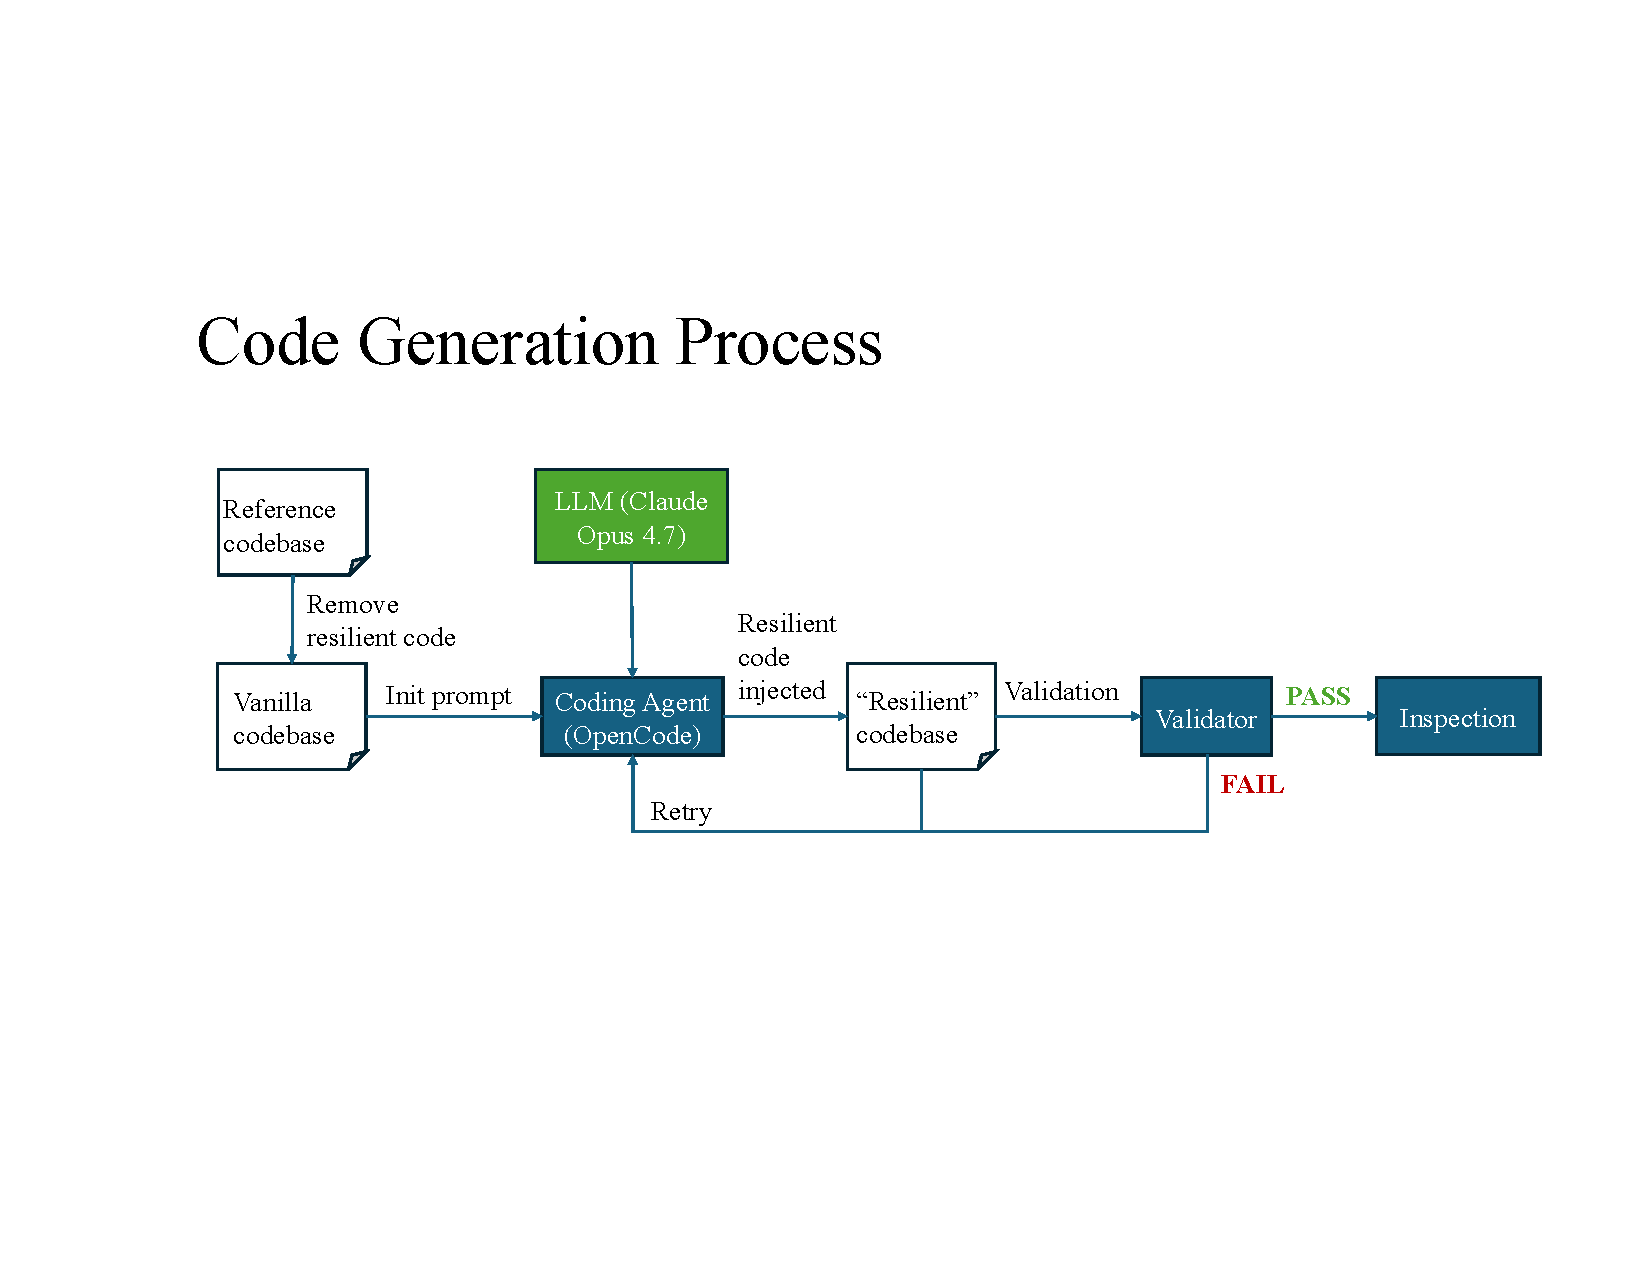
\includegraphics[width=\linewidth, trim={100 200 60 220}, clip]{Figures/code-gen-process.pdf}
    \caption{End-to-end LLM-driven pipeline for adding checkpoint/restart resilience to an
             unmodified MPI application.}
    \label{fig:code-gen-process}
\end{figure}

\medskip
\noindent\textbf{Experimental Pipeline.}
Figure~\ref{fig:code-gen-process} sketches the end-to-end pipeline we use to test whether
a frontier LLM can autonomously add checkpoint/restart resilience to an MPI scientific
code.  We start by stripping the upstream source of any existing resilience logic to
produce a \emph{vanilla codebase}; this is the only artifact the LLM ever sees.  We then
drive an iterative code-generation loop, in which each iteration executes two phases in
sequence with no human in the loop.

\begin{enumerate}[topsep=0pt,itemsep=0pt,leftmargin=*]
    \item \textbf{Code Generation.} We give Anthropic's Claude Opus 4.7~\cite{claude}, invoked through the \texttt{opencode} coding-agent CLI~\cite{opencode}, the vanilla source tree plus a fixed instruction prompt that asks it to use VeloC~\cite{veloc} (a multi-level checkpoint/restart runtime designed for HPC) to protect the application against process failure. The agent issues \texttt{read}/\texttt{edit} tool calls on the source tree and writes a modified copy we call the \emph{resilient codebase}, which must preserve the vanilla code's functional behavior while adding fault tolerance. The prompt also asks the agent to log its reasoning, intended action, observed result, and next step at every iteration, giving us a per-step transcript of the transformation.

    \item \textbf{Validation.} An independent validator builds the resilient codebase and, if the build succeeds, runs it under two scenarios. \emph{Failure-free execution} confirms the modified code still produces output equivalent to the vanilla under tolerance, ensuring the functional contract is intact. \emph{Failure-injected execution} kills one rank mid-run, re-launches the binary, and checks four conditions: (i)~at least one checkpoint file was written before the kill; (ii)~the harness actually delivered the failure (no spurious early exit); (iii)~the post-restart output matches the vanilla, confirming the checkpoint plus recovery path reproduces the intended results; and (iv)~end-to-end wall time stays meaningfully below a full restart-from-scratch, evidence the checkpoint cadence is operationally useful.
\end{enumerate}

\noindent
If any check fails or the run times out, the loop iterates: the agent receives the original prompt, its previous resilient code, and the validator's structured feedback (build log, execution stdout/stderr, per-condition pass/fail flags) and is asked to produce a corrected version. Each application is allowed up to ten iterations; if the validator passes before that cap, the resulting code is promoted to the inspection phase analyzed in \S\ref{sec:findings}.

% \subsection{Metrics}

\medskip
\noindent\textbf{Metrics and Configurations.}
The inspection phase collects four metrics per application:
(i)~\emph{Code generation time}: cumulative wall time of the LLM/validator loop, including both the agent's thinking time and the validator's build/run time;
(ii)~\emph{Total tokens}: input plus output tokens consumed across all iterations, a direct proxy for API spend;
(iii)~\emph{End-to-end execution time}: wall time of one application run under each scenario, quantifying both instrumentation overhead and recovery cost; and
(iv)~\emph{Per-frame checkpoint footprint}: bytes written by a single checkpoint event, capturing the storage cost of the chosen state coverage.
All measurements were collected on a single development host with 4~MPI ranks per application. Per-app input arguments were tuned so one failure-free run takes 60--200~s, short enough to keep the iterative loop tractable yet long enough for failure injection to produce meaningful checkpoint, recovery, and output signals. For every (application, scenario) cell we run three independent trials and report the mean. All runs use the latest released version of VeloC~\cite{veloc}.


% =====================================================================
\section{Key Findings}
\label{sec:findings}


% \subsection{How the Agent Enables Resiliency}
% \label{sec:reasoning}

We trace what actually happens inside the iterative loop, distilled from the per-iteration \texttt{opencode\_stdout} transcripts that record the agent's reasoning and actions step by step. Across all seventeen applications the transcripts reveal the \emph{same four-phase procedure}, applied with very few app-specific deviations:

\begin{enumerate}[topsep=0pt,itemsep=0pt,leftmargin=12pt]
    \item \textbf{Reconnaissance.}  The agent locates the application's main timestep loop, starting from the entry-point file (\texttt{main.cpp} or equivalent) and following function calls inward.  It also locates the VeloC installation on disk and reads the VeloC documentation to learn the API it will need.
    \item \textbf{Critical-state identification.}  The agent walks the application's central data structure field by field and labels each field as either \emph{rebuildable} (the input deck plus the application's own initialization code can recreate it) or \emph{evolving} (the value changes inside the timestep loop and therefore must be saved).
    % Every rejection is justified in writing in the transcript.
    \item \textbf{Implementation.} The agent wires VeloC into the application: it initializes the runtime at startup, declares memory regions of evolving fields to checkpoint, calls the checkpoint primitive at a chosen cadence inside the timestep loop, and adds a startup branch that detects an existing checkpoint, restores the saved state, and resumes the loop from the saved counter.
    \item \textbf{Self-review.} The agent walks the change diff and lists the corner cases it has thought through (first-ever run, partial checkpoint write, restart-counter collisions, halo cells, RNG state, and so on), justifying how each is handled before declaring the iteration ready for validation.
\end{enumerate}

\begin{figure}[t]
  \centering
  
\includegraphics[width=\columnwidth]{Figures/fast_tier_iter_walltime.pdf}
  \caption{Time consumed by the LLM iterative loop to produce a working checkpoint/restart implementation, per app.
  % Bars are stacked into LLM code generation (dark blue, bottom) and validation (light blue, top), summed across all iterations.
  }
  \label{fig:walltime}
\end{figure}

This procedure successfully transformed \textit{all} seventeen vanilla codebases into resilient ones. We walk through each application below in roughly increasing order of state complexity, then summarize the cross-cutting design choices that recur across the suite.

\paragraph{HPCG (2 iterations to PASS)}
HPCG is the suite's simplest case: each CG solve starts from the same zeroed initial vector and no state carries over between solves, so the only critical state is a counter plus the residual array. The agent rejected saving the sparse matrix, multigrid hierarchy, and per-solve scratch vectors as deterministically rebuildable from the input dimensions.

\paragraph{CoMD (2 iterations to PASS)}
CoMD is harder than HPCG because state evolves inside the timestep loop: atoms migrate between MPI subdomains every step, so the per-rank atom list (positions, momenta, forces, identifiers) plus a small link-cell bookkeeping array changes continuously. Everything else (simulation box, species table, potentials, link-cell geometry) is fixed at startup, and halo cells are repopulated on the first post-restart timestep by CoMD's own halo-exchange. The agent saved the atom arrays plus the loop counter and skipped halos.

\paragraph{OpenLB (1 iteration to PASS)}
OpenLB stores far more data per process than CoMD, and that data is tangled inside an internal object whose layout would be tedious and error-prone to list by hand. Conveniently, OpenLB already provides three helper methods designed for sending the object between processes (return its size, pack it into a buffer, unpack it from a buffer); after an intensive search over the codebase, the agent found and reused them as a black-box serialization, so it never needed to know what the object actually contains.

\paragraph{SPARTA (2 iterations to PASS)}
SPARTA introduces a new wrinkle: per-rank particle counts vary because particles drift between ranks every timestep, ruling out fixed-size memory regions. The agent used VeloC's file-based API to write a small structured payload per rank (timestep counter, simulation-time scalars, particle count, particle array, RNG state) and skipped the static grid topology, species tables, and master RNG.

\paragraph{Athena++ (4 iterations to PASS)}
Athena++ raises the stakes again: its state lives in an evolving AMR mesh tree plus a long list of conditional physics arrays, so field-by-field enumeration would have been both labor-intensive and high-risk. The agent instead implemented a writer/reader pair dedicated to Athena++'s mesh format to dump and reconstruct the critical state from disk.

\paragraph{LAMMPS (7 iterations to PASS)}
LAMMPS has the most complex state in the suite. Its atoms move between ranks as in SPARTA, but it also tracks two things no other app does: bonds and angles that link atoms together (a graph the checkpoint must keep consistent after migration), and many small pieces of state owned by whichever optional physics modules the user turns on (each one keeps its own counters and random-number state).

\paragraph{PRK\_Stencil (2 iterations to PASS)}
PRK\_Stencil resembles HPCG in spirit but evolves real per-step state: a 2D stencil sweeps a single working array, so the only critical state is the iteration counter and the array itself. Iteration~1 wired the \texttt{VELOC\_Mem\_protect} calls but failed validation because \texttt{veloc.cfg} sat under \texttt{Stencil/} where the build system did not stage it; iteration~2 was a one-line config relocation to the project root.

\paragraph{Smilei (3 iterations to PASS)}
Smilei is a relativistic PIC code with a deeply nested particle/field hierarchy, so the agent declined to enumerate it field by field. Instead it dumped the three integrators that drive the loop (\texttt{itime}, \texttt{time\_prim}, \texttt{time\_dual}) as a small fixed-size byte payload through VeloC's file-based API and let Smilei's own initialization rebuild the rest. Iterations~2 and~3 were build-system fixes: missing \texttt{-lveloc} in the C++ link line surfaced as undefined-symbol errors that took two passes to localize to the right \texttt{LDFLAGS} block in the bespoke makefile.

\paragraph{SPPARKS (2 iterations to PASS)}
SPPARKS is closer to LAMMPS than to HPCG: a rejection-kinetic-Monte-Carlo lattice solver carries a non-trivial mix of evolving state (current time, per-site spin array, accept/reject counters, Marsaglia RNG state). The agent registered each component with \texttt{VELOC\_Mem\_protect} and explicitly excluded the static lattice topology and the master RNG seed as deterministically rebuildable. Iteration~2 was a config-placement fix mirroring the PRK\_Stencil pattern.

\paragraph{Nyx (5 iterations to PASS)}
Nyx is the first AMReX-based app in the suite and exposes the difficulty of integrating with a heavy C++ template framework: critical state lives in distributed \texttt{MultiFab} objects whose extents change with the AMR hierarchy. The agent chose memory-protect over a coordinator approach, writing helper functions that walk each \texttt{MultiFab} and register its underlying float arrays with VeloC. The five-iteration arc was almost entirely build-system pain: header-include order, AMReX namespace resolution, and CMake integration each cost an iteration before the resilient binary linked cleanly.

\paragraph{ROSS (3 iterations to PASS)}
ROSS is a parallel discrete-event simulator whose recovery semantics differ from every other app in the suite: after restart the global virtual time (GVT) machinery must not double-count events committed before the failure. The agent serialized a small POD struct (current GVT, per-rank event counters, anti-message bookkeeping) through VeloC's file-based API and added a post-restore correction step that re-establishes the cumulative-statistics baseline. Iterations~2 and~3 closed two related bugs in that correction path that surfaced as biased steady-state event-rate measurements.

\paragraph{SW4lite (2 iterations to PASS)}
SW4lite is a 4th-order seismic wave-propagation kernel whose state is three rolling time-step buffers (\texttt{Um}, \texttt{U}, \texttt{Up}) plus the step counter. The agent dumped the three buffers and the counter as a single opaque payload via VeloC's file-based API rather than registering each array individually, because the buffers are allocated as flat C arrays with sizes already known to the host code. Iteration~2 was a CMake placement fix: the agent had added VeloC linkage to the wrong \texttt{add\_executable} target.

\paragraph{QMCPACK (3 iterations to PASS)}
QMCPACK runs Monte Carlo electronic-structure samples whose physics state is owned by an internal walker manager that the agent judged too risky to dissect; instead it preserved a minimal coordinator (the QMC iteration counter via \texttt{VELOC\_Mem\_protect}) plus a small file-based blob holding the random-number-generator state. This is why QMCPACK's per-frame checkpoint is only 40 bytes in \autoref{fig:frame}: physics state is regenerated by QMCPACK's own initialization rather than carried across the recovery boundary. Iteration~3 fixed a comparator that had been keying on a banner-style \texttt{completed successfully} string; the agent rewrote it to compare the recovered reference energy within tolerance \(0.01\).

\paragraph{CLAMR (3 iterations to PASS)}
CLAMR is an adaptive-mesh shallow-water hydro code where each rank owns a different cell count, so fixed-size memory regions were ruled out. The agent dumped per-rank arrays \texttt{H} (height), \texttt{U}, \texttt{V} (momenta), and the active cell count through VeloC's file-based API. Iterations~2 and~3 resolved two cascading restore-time bugs: a per-rank size mismatch when ranks resized between checkpoints, and a conflict with CLAMR's L7 communication library, which holds MPI state that had to be re-initialized after the VeloC restore call.

\paragraph{HyPar (3 iterations to PASS)}
HyPar is a finite-difference hyperbolic-parabolic solver whose critical state is the conserved-variable array \texttt{u[]} plus integrator scratch buffers and the step counter; the agent registered each via \texttt{VELOC\_Mem\_protect} following the HPCG/CoMD template. Iterations~2 and~3 were build and runtime configuration fixes: integrating VeloC into HyPar's CMake graph took one iteration, and a \texttt{getenv}-based runtime path lookup that returned NULL inside the validator's process took another to diagnose and replace with an explicit config path.

\paragraph{WarpX (5 iterations to PASS)}
WarpX is the largest codebase in the suite (627K LOC, AMReX-based PIC) and ships full native checkpoint/restart through the \texttt{amr.restart=<chkdir>} input parameter. The agent first attempted a memory-protect approach mirroring Nyx, registering top-level \texttt{MultiFab} buffers, but iteration~3 logs show it abandoned that path after concluding that capturing all conditional physics modules (electromagnetic solvers, particle species, embedded boundaries) would be intractable. The pivot was decisive: VeloC keeps only the step counter and the native checkpoint directory name (24~bytes per frame in \autoref{fig:frame}), and on restart the agent\textquotesingle s shim rewrites the \texttt{amr.restart} input and re-execs WarpX through its own restart entry point. Iterations~4 and~5 hardened that shim against partially-written checkpoint directories.

\paragraph{SAMRAI (1 iteration to PASS)}
SAMRAI converged in a single iteration because it ships a first-class \texttt{tbox::RestartManager} infrastructure that already serializes every registered \texttt{Database} object to disk. The agent detected this immediately and selected the same coordinator pattern as WarpX: VeloC tracks only the step counter and the \texttt{RestartManager}\textquotesingle s output directory (304~bytes per frame), and on restart hands control to \texttt{RestartManager::openRestartFile} rather than reconstructing patch state itself. SAMRAI is the strongest evidence in the suite that when an app's own restart abstractions are clean and discoverable, the agent recognizes them on the first pass and writes minimal coordinator code rather than reimplementing them.

\paragraph{Cross-cutting observations}
Three patterns recur across all seventeen apps. First, the agent always starts from a \emph{small} state-coverage set rather than a conservative \emph{everything} one: it picks the few fields that actually evolve, defends every rejection in writing, and only adds coverage if validator feedback forces it. This is the proximate reason failure-free overhead is essentially zero across the suite. Second, the agent's willingness to \emph{reuse application-specific infrastructure} (OpenLB's serialize methods, Athena++'s restart-file reader, WarpX's \texttt{amr.restart}, SAMRAI's \texttt{RestartManager}, LAMMPS's \texttt{restart}/\texttt{read\_restart} commands) is the single biggest predictor of fast convergence: nine of the seventeen apps converge in $\le 3$ iterations because the agent found and reused such infrastructure rather than re-implementing it. Third, when the validator reports a failure the agent treats it as structured triage: read the exact error, form one hypothesis, investigate it before forming the next, and only then propose a fix. Failures cluster into three causes: configuration misplacement (e.g., \texttt{veloc.cfg} not at the path the validator probes; fixed in 1--2 iterations on PRK\_Stencil, SPPARKS, HyPar, QMCPACK), build/CMake integration issues (Athena++, SW4lite, HyPar, Nyx), and post-restart determinism drift (LAMMPS atom-owner ordering, which required six hypothesis-elimination iterations).

% =====================================================================
% \subsection{Time to Construct Resilient Code}
\medskip
\noindent\textbf{Time to Construct Resilient Code.}
The iterative loop consumed 12.7~hours total across the seventeen apps, averaging 45~minutes per app, with a $\sim$\,$8.5\times$ spread between the fastest (HPCG, 14~min) and the slowest (WarpX, 121~min). Figure~\ref{fig:walltime} decomposes per-app loop time into LLM code generation (dark blue, bottom) and validation (light blue, top): \emph{code generation dominates on every app}, taking a median of 61\% of the total (range 50--84\%).

The bar shapes track the difficulty ordering. Small fixed-state apps (HPCG 14~min, CoMD 22~min, OpenLB 21~min) sit at the bottom because their critical state is small and the iteration~1 design was structurally correct, with at most a one-line operational fix on iteration~2. Medium-complexity apps (SPARTA 64~min, Athena++ 87~min, LAMMPS 92~min) require multiple iterations to capture richer state surfaces. The largest codebases (WarpX 121~min, Nyx 55~min, ROSS 51~min, SW4lite 54~min) dominate the chart because either their per-rank state is intricate or recovery semantics required multi-iteration debugging.

% \subsection{Token Cost}

\begin{figure}[t]
  \centering
  
\includegraphics[width=\columnwidth]{Figures/fast_tier_iter_tokens.pdf}
  \caption{Total Claude Opus 4.7 tokens consumed by the iterative loop, per app.
  % Bars are stacked into input tokens (blue, bottom; source code, prompt, and validator feedback the agent reads) and output tokens (amber, top; code edits the agent writes), summed across all iterations.
  }
  \label{fig:tokens}
\end{figure}

\medskip
\noindent\textbf{Token Cost.}
Total tokens across the seventeen apps sum to 86.1~M (average 5.1~M per app), corresponding to roughly \$200--1500 in API spend at current frontier-model rates \cite{anthropic_pricing}. \autoref{fig:tokens} spans $\sim$\,$85\times$, from CoMD's 0.28~M up to WarpX's 23.7~M.

Token cost correlates only loosely with code generation time. WarpX tops the chart at 23.7~M because its 553K-line PIC+AMR codebase requires the agent to scan a substantial portion of the source to find the relevant integrator, particle, and field hooks. OpenLB at 7.8~M converged in a single iteration but still needed extensive scanning of its 338K-line source tree to discover the built-in serialize methods. CoMD sits at the bottom (0.28~M) because of its small 5.6K-LOC codebase and small critical state. The token total is dominated by source-tree size, not by iteration count.

The stacked decomposition shows input tokens account for roughly 99\% of every bar (the agent reads orders of magnitude more text than it writes): \emph{input-context size is the dominant token cost driver}, so pre-summarizing or chunking large source trees would translate directly into spend reductions, especially on the largest apps (WarpX, QMCPACK 532K, SAMRAI 598K, Nyx 441K) where exploration substantially exceeds eventual edits.

% \subsection{Overhead: Runtime and Storage}
% \label{sec:findings-failure-free-overhead}

\begin{figure}[t]
  \centering
  
\includegraphics[width=\columnwidth]{Figures/fast_tier_compare_walltime_failure_free.pdf}
  \caption{Per-app average execution time under the failure-free scenario.}
  \label{fig:ff}
\end{figure}

\begin{figure}[t]
  \centering
  
\includegraphics[width=\columnwidth]{Figures/fast_tier_compare_checkpoint_per_frame.pdf}
  \caption{Payload size of a full recoverable checkpoint.}
  \label{fig:frame}
\end{figure}

\medskip
\noindent\textbf{Overhead: Runtime and Storage.}
\autoref{fig:ff} shows an important result: \textit{the LLM-generated checkpoint instrumentation imposes essentially zero failure-free overhead}. Fourteen of seventeen apps fall within $\pm 2\%$ of vanilla wall time (range $-1.1\%$ for CLAMR to $+1.9\%$ for SW4lite), well inside measurement noise. Two apps fall in the moderate band (Nyx $+2.9\%$, SAMRAI $+2.8\%$). Only PRK\_Stencil shows a larger overhead at $+9.2\%$, attributable to the chosen checkpoint cadence on its tight stencil loop. The LLM bars track the upstream reference closely on every app, so the generated code matches a human-engineered native implementation.

\autoref{fig:frame} shows full-checkpoint sizes spanning many orders of magnitude, from per-frame footprints of tens of bytes up to hundreds of megabytes (CoMD's 194~MB full per-rank atom array; PRK\_Stencil's 257~MB grid). The smallest LLM checkpoints (24~B WarpX, 256~B Smilei, 284~B Nyx, 304~B SAMRAI, 312~B ROSS, 420~B QMCPACK, 744~B HyPar) reflect the \emph{coordinator pattern} described in \S\ref{sec:reasoning}: on these apps the LLM defers physics-state preservation to the application's native checkpoint mechanism and writes only a step counter plus the native-checkpoint directory pointer through VeloC, which is sufficient for VeloC to coordinate the restart. LLM and reference agree on the order of magnitude on most apps; where they diverge (e.g.\ HPCG LLM~66~KB vs.\ reference~6~KB; OpenLB LLM~3~MB vs.\ reference~157~KB) the LLM is more conservative, persisting diagnostic accumulators the reference recomputes on restart. \textbf{[TODO: 4 of 17 reference checkpoints (Nyx, SAMRAI, SPPARKS, WarpX) cannot be measured because their upstream native checkpoint formats (AMReX-native, HDF5, custom binary) are not introspected by our metric collector; bars for those references render as ``n/a''. Resolution: extend the metric collector with format-specific introspection.]}

% \subsection{Resiliency}

\begin{figure}[t]
  \centering
  
\includegraphics[width=\columnwidth]{Figures/fast_tier_compare_walltime_failure_injected.pdf}
  \caption{Per-app end-to-end execution time with a failure injected mid-run.
  % The binary re-launches after failures. LLM-modified and reference binary detect existing checkpoint files and resume while vanilla has to restart from scratch.
  }
  \label{fig:once}
\end{figure}

\medskip
\noindent\textbf{Resilience.}
\autoref{fig:once} shows per-app end-to-end runtime when the validator kills one MPI rank mid-run, then restarts the app. The LLM runtime sits close to the reference on most apps, with recovery ratios (once / failure-free) clustering tightly between 1.01$\times$ and 1.09$\times$ for fourteen of seventeen apps. Both the LLM and reference recover within roughly one third of the wall-clock penalty paid by the vanilla baseline, which has no checkpoint protection and must restart from scratch. Two outliers warrant note: SAMRAI (LLM ratio 1.50$\times$) and SPPARKS (reference ratio 1.51$\times$) effectively restart-from-scratch because their LLM checkpoint preserves only metadata (SAMRAI) or because the upstream code lacks native checkpoint support (SPPARKS). \textbf{[TODO: OpenLB's LLM once-cell summary in the chart is computed from a stale n=3 aggregate (mean 205~s) that does not include the two clean post-extension runs (true mean 173~s, median 126~s); re-aggregate the OpenLB\_baseline summary block from the n=5 raw runs before camera-ready.]} Apart from these, the chart is operational evidence the LLM-generated code does real recovery work: detecting checkpoint files, restoring state, and resuming with overhead bounded by the checkpoint cadence rather than by the size of the original computation.

% =====================================================================
\section{Conclusion and Future Work}
\label{sec:conclusion}
% =====================================================================

This paper investigates whether frontier LLM coding agents can automate end-to-end checkpoint/restart integration for existing MPI scientific applications. Across seventeen applications with diverse domains (1K to 627K LOC), data structures, and checkpointing patterns, the agent generated working resilient implementations without human intervention after the initial prompt. The generated code achieved near-zero failure-free overhead on fourteen of seventeen applications, recovered from injected failures with performance close to upstream native implementations on every app where the comparison is available, and converged in under two hours per application. These results suggest that LLM-driven resilience engineering can substantially reduce the expert effort required to add production-grade fault tolerance to a meaningful subset of HPC applications.

Future work should improve the robustness, scalability, and usability of this approach. Specialized pipelines with resilience-specific skills, source-code summarization, checkpoint-state analysis, and targeted validation feedback could reduce cost and improve reliability. Broader evaluations are needed for repeated failures, realistic I/O environments, multi-node executions, and applications with more irregular or distributed state. Finally, generated checkpoint code should become easier to audit, maintain, and integrate into production workflows so that automated resilience generation can be used safely in practice.

\bibliographystyle{IEEEtran}
\bibliography{references}

% \section*{References}

% Please number citations consecutively within brackets \cite{b1}. The 
% sentence punctuation follows the bracket \cite{b2}. Refer simply to the reference 
% number, as in \cite{b3}---do not use ``Ref. \cite{b3}'' or ``reference \cite{b3}'' except at 
% the beginning of a sentence: ``Reference \cite{b3} was the first $\ldots$''

% Number footnotes separately in superscripts. Place the actual footnote at 
% the bottom of the column in which it was cited. Do not put footnotes in the 
% abstract or reference list. Use letters for table footnotes.

% Unless there are six authors or more give all authors' names; do not use 
% ``et al.''. Papers that have not been published, even if they have been 
% submitted for publication, should be cited as ``unpublished'' \cite{b4}. Papers 
% that have been accepted for publication should be cited as ``in press'' \cite{b5}. 
% Capitalize only the first word in a paper title, except for proper nouns and 
% element symbols.

% For papers published in translation journals, please give the English 
% citation first, followed by the original foreign-language citation \cite{b6}.

% \begin{thebibliography}{00}
% \bibitem{b1} G. Eason, B. Noble, and I. N. Sneddon, ``On certain integrals of Lipschitz-Hankel type involving products of Bessel functions,'' Phil. Trans. Roy. Soc. London, vol. A247, pp. 529--551, April 1955.
% \bibitem{b2} J. Clerk Maxwell, A Treatise on Electricity and Magnetism, 3rd ed., vol. 2. Oxford: Clarendon, 1892, pp.68--73.
% \bibitem{b3} I. S. Jacobs and C. P. Bean, ``Fine particles, thin films and exchange anisotropy,'' in Magnetism, vol. III, G. T. Rado and H. Suhl, Eds. New York: Academic, 1963, pp. 271--350.
% \bibitem{b4} K. Elissa, ``Title of paper if known,'' unpublished.
% \bibitem{b5} R. Nicole, ``Title of paper with only first word capitalized,'' J. Name Stand. Abbrev., in press.
% \bibitem{b6} Y. Yorozu, M. Hirano, K. Oka, and Y. Tagawa, ``Electron spectroscopy studies on magneto-optical media and plastic substrate interface,'' IEEE Transl. J. Magn. Japan, vol. 2, pp. 740--741, August 1987 [Digests 9th Annual Conf. Magnetics Japan, p. 301, 1982].
% \bibitem{b7} M. Young, The Technical Writer's Handbook. Mill Valley, CA: University Science, 1989.
% \end{thebibliography}
% \vspace{12pt}
% \color{red}
% IEEE conference templates contain guidance text for composing and formatting conference papers. Please ensure that all template text is removed from your conference paper prior to submission to the conference. Failure to remove the template text from your paper may result in your paper not being published.

\end{document}
